\documentclass{article}
\usepackage{pdfpages}
\usepackage{pdflscape}
\usepackage[utf8]{inputenc}
\usepackage{mathcomp}
\title{Sprawozdanie z Laboratorium 1. \\ \large Pomiary wielkości geometrycznych \\ Prawo Ohma}
\author{Piotr Lewandowski \and Dymitr Lubczyk \and Krzysztof Tabeau }
\date{15.03.2020}

\usepackage{natbib}
\usepackage{graphicx}

%%%
% https://docs.google.com/spreadsheets/d/1a7a6zwNaL0n1_6OelipUeUKeIgoOb76PJvlL9x7z3Tw
%%%

%language
\usepackage[T1]{fontenc}
\usepackage[polish]{babel}
\usepackage[utf8]{inputenc}

\begin{document}

\maketitle

\section{Pomiar wielkości geometrycznych}

\subsection{Wstęp}
Celem przeprowadzonego ćwiczenia było zapoznanie się z metodyką poprawnego mierzenia wielkości fizycznych. W tym celu dokonaliśmy z użyciem śruby mikrometrycznej 10 pomiarów średnicy kuli, oraz przy pomocy suwmiarki 3 pomiarów długości, szerokości i wysokości prostopadłościanu. Wyniki pomiarów są zawarte w poniższych tabelach.

\begin{table}[h!]
\centering
\begin{tabular}{|l|}
\hline
d     \\ \hline
15,35 \\ \hline
15,38 \\ \hline
15,39 \\ \hline
15,35 \\ \hline
15,33 \\ \hline
15,32 \\ \hline
15,36 \\ \hline
15,35 \\ \hline
15,40 \\ \hline
15,41 \\ \hline
\end{tabular}
\caption{Średnica kuli (w milimetrach)}
\end{table}


\begin{table}[h!]
\centering
\begin{tabular}{|l|l|l|}
\hline
a         & b         & c         \\ \hline
40,08     & 29,40     & 3,50      \\ \hline
40,10     & 29,38     & 3,70      \\ \hline
40,08     & 29,40     & 3,70      \\ \hline
\end{tabular}
\caption{Długość, szerokość oraz wysokość prostopadłościanu (w milimetrach)}
\end{table}

\subsection{Wyznaczanie niepewności pomiaru}

Niepewność pomiaru dzielimy na dwa typy: typ A, oparty na metodzie statystycznego opracowywania danych oraz typ B, zależny od osądu badacza, na który wpływ ma m.in. niepewność pomiarowa urządzenia.

\subsubsection{Średnica kuli}
Przy mierzeniu średnicy kuli, niepewność typu B wynosiła, dla najmniejszej podziałki rozmiaru $0.01mm$.
$$ u_B(d) = \frac{0.01}{\sqrt{3}} = 0.0058 $$ 
\\
Niepewność typu A wyliczyliśmy w następujący sposób:
$$ \overline{d} = \sum_1^{10} d_i = 15.364 $$
$$ u_A(d) = \sqrt{ \frac{\sum_1^{10} (d_i - \overline{d})^2 }{10 (10-1)}} = 0.0095 $$
\\
Ostatecznie wyznaczona średnica kuli, z uwzględnieniem niepewności to:
$$ u(d) = \sqrt{u_A(d)^2 + u_B(d)^2} = 0.011 $$
$$ d = 15.364(11) [mm] $$ 

\subsubsection{Objętość prostopadłościanu}
Wszystkie pomiary zostały wykonane z wykorzystaniem tego samego narzędzia, więc w tym przypadku niepewność typu B, dla najmniejszej podziałki rozmiaru $0.02mm$, jest równa:
$$ u_B(a) = u_B(b) = u_B(c) = \frac{0.02}{\sqrt{3}} = 0.012 $$
\\
Szukamy objętości zadanej wzorem $ V = a b c$, więc niepewność możemy wyliczyć korzystając ze wzoru:
$$ u(V) = \sqrt{
    \left(\frac{\partial V}{\partial a}u(a)\right)^2 
    + \left(\frac{\partial V}{\partial b}u(b)\right)^2
    + \left(\frac{\partial V}{\partial c}u(c)\right)^2
} = 0.44 [mm^3] $$
\\
Ostateczny wynik to:
$$ V = 4281.09(44) [mm^3] $$

\clearpage

\section{Prawo Ohma}

\subsection{Wstęp}
Celem drugiej części laboratorium było wyznaczenie rezystancji oporników korzystając z Prawa Ohma. Zmierzyliśmy napięcie i natężenie na każdym z oporników $ R_1, R_2, R_3, R_4 $ podłączanych zgodnie z poniższym schematem do analogowego woltomierza i cyfrowego amperomierza. Pomiary dla oporników $ R_1, R_2, R_3 $ zostały przeprowadzone jednokrotnie, a pomiary dla opornika $ R_4 $ wykonaliśmy 15 razy.

\begin{figure}[h!]
\centering
\includegraphics[scale=0.6]{obwód.png}
\caption{Schemat obwodu}
\end{figure}

\subsection{Teoria}
Prawo Ohma mówi o tym, że stosunek natężenia prądu stałego płynącego przez przewodnik jest wprost proporcjonalne do napięcia przyłożonego do jego końców. 
$$ I \sim U $$
\\
Regresja liniowa to w modelowaniu statystycznym, metody oparte o liniowe kombinacje zmiennych i parametrów dopasowujących model do danych. Dopasowana linia regresji reprezentuje oszacowaną wartość oczekiwaną zmiennej y przy różnych wartościach zmiennych x.
\\\\
W naszym przypadku użyliśmy regresji liniowej i prawa Ohma do wyznaczenia oporu opornika R4, przy wielokrotnych pomiarach napięcia i natężenia w rożnych zakresach pomiarowych.


\clearpage


\subsection{Wyniki Pomiarów}

\begin{table}[h!]
\centering
\begin{tabular}{|l|l|l|l|}
\hline
I {[}mA{]} & U {[}V{]} & zak. I {[}mA{]} & zak. U {[}V{]} \\ \hline
1,347      & 0,52      & 2               & 1              \\ \hline
1,9        & 0,72      & 2               & 1              \\ \hline
3,26       & 1,3       & 20              & 3              \\ \hline
5,43       & 2,1       & 20              & 3              \\ \hline
6,86       & 2,7       & 20              & 3              \\ \hline
8,18       & 3,2       & 20              & 10             \\ \hline
9,02       & 3,6       & 20              & 10             \\ \hline
10,85      & 4,2       & 20              & 10             \\ \hline
13,03      & 5         & 20              & 10             \\ \hline
14,92      & 5,8       & 20              & 10             \\ \hline
17         & 6,6       & 20              & 10             \\ \hline
21,8       & 8,6       & 200             & 10             \\ \hline
25,8       & 10,2      & 200             & 30             \\ \hline
31,5       & 12,5      & 200             & 30             \\ \hline
41,1       & 15,4      & 200             & 30             \\ \hline
\end{tabular}
\caption{Napięcie i natężenie zmierzone na oporniku $ R_4 $}
\end{table}

\begin{table}[h!]
\centering
\begin{tabular}{l|l|l|l|l|}
\cline{2-5}
                         & I {[}mA{]} & U {[}V{]} & zak. I {[}mA{]} & zak. U {[}V{]} \\ \hline
\multicolumn{1}{|l|}{$ R_1 $} & 43,2       & 2,45      & 200             & 3              \\ \hline
\multicolumn{1}{|l|}{$ R_2 $} & 23         & 2,25      & 200             & 3              \\ \hline
\multicolumn{1}{|l|}{$ R_3 $} & 25,3       & 2,6       & 200             & 10             \\ \hline
\end{tabular}
\caption{Wyniki pomiarów dla oporników $ R_1, R_2, R_3 $ }
\end{table}

\clearpage

\subsection{Wyznaczanie rezystancji oporników $ R_1, R_2, R_3 $}
W przypadku jednokrotnego pomiaru uwzględniamy jedynie niepewność typu B, więc dla wszystkich trzech oporników
$$ u(U) = u_B(U) = \frac{k z}{100} * \frac{1}{\sqrt{3}} $$
Gdzie $k$ to klasa woltomierza, a $z$ to aktualny zakres pomiarowy.
$$ u(I) = u_B(I) = 0.05 w + 0.01 z $$
Gdzie $w$ to wynik pomiaru, a $z$ to aktualny zakres pomiarowy.
$$ u(R) = \sqrt{
    \left(\frac{\partial R}{\partial U}u(U)\right)^2 
    + \left(\frac{\partial R}{\partial I}u(I)\right)^2
} = \sqrt{
    \left(\frac{1}{I}u(U)\right)^2 
    + \left(\frac{-U}{I^2}u(I)\right)^2
} $$

\begin{table}[h!]
\centering
\begin{tabular}{|l|l|l|l|}
\hline
$u_b(I)[mA]$    & $u_b(U)[V]$      & $u(R)[\Omega]$        & $r[\Omega]$           \\ \hline
3,31    & 0,017   & 4,37  & 56,71  \\ \hline
2,30    & 0,017   & 9,83  & 97,83  \\ \hline
2,42    & 0,058   & 10,09 & 102,77 \\ \hline
\end{tabular}
\caption{Niepewności pomiarowe dla oporników $ R_1, R_2, R_3 $ }
\end{table}

Ostatecznie zmierzone wartości rezystancji dla tych oporników to:
$$ R_1 = 56.71(4.37) [\Omega] $$
$$ R_2 = 97.82(9.83) [\Omega] $$
$$ R_3 = 102.77(10.09) [\Omega] $$

\subsection{Wyznaczanie rezystancji opornika $ R_4 $}
Z powodu mierzenia pomiarów w różnych zakresach, odchylenie standardowe wyszło bardzo duże zarówno dla napięcia i natężenia, co skutkuje w dużych niepewnościach dla tych danych. Jako że błąd typu B w niektórych przypadkach jest o rząd niższy niż błąd typu A, jest on pomijany w wyliczeniach.
Obliczenie niepewności oporu zostało wykonane metodami statystycznymi w arkuszu kalkulacyjnym. 
Poniżej przedstawiamy nasze wyniki.
\\
$$ R = 387(2.6) [\Omega] $$
$$ u_A(I) = 2.98 $$
$$ u_A(U) = 1.15 $$

\begin{table}[h!]
\centering
\begin{tabular}{|l|l|l|l|}
\hline
$u_b(I)$ & $u_b(U)$ & $u(I)$ & $u(U)$ \\ \hline
0,079   & 0,0058  & 2,98 & 1,15 \\ \hline
0,11    & 0,0058  & 2,98 & 1,15 \\ \hline
0,28    & 0,017   & 2,99 & 1,15 \\ \hline
0,39    & 0,017   & 3,01 & 1,15 \\ \hline
0,46    & 0,017   & 3,02 & 1,15 \\ \hline
0,52    & 0,058   & 3,03 & 1,15 \\ \hline
0,57    & 0,058   & 3,03 & 1,15 \\ \hline
0,66    & 0,058   & 3,05 & 1,15 \\ \hline
0,77    & 0,058   & 3,08 & 1,15 \\ \hline
0,86    & 0,058   & 3,10 & 1,15 \\ \hline
0,97    & 0,058   & 3,13 & 1,15 \\ \hline
2,24    & 0,058   & 3,73 & 1,15 \\ \hline
2,44    & 0,17    & 3,86 & 1,16 \\ \hline
2,73    & 0,17    & 4,04 & 1,16 \\ \hline
3,21    & 0,17    & 4,38 & 1,16 \\ \hline
\end{tabular}
\caption{Niepewności pomiarów dla opornika $ R_4 $}
\end{table}



\begin{figure}[h!]
\centering
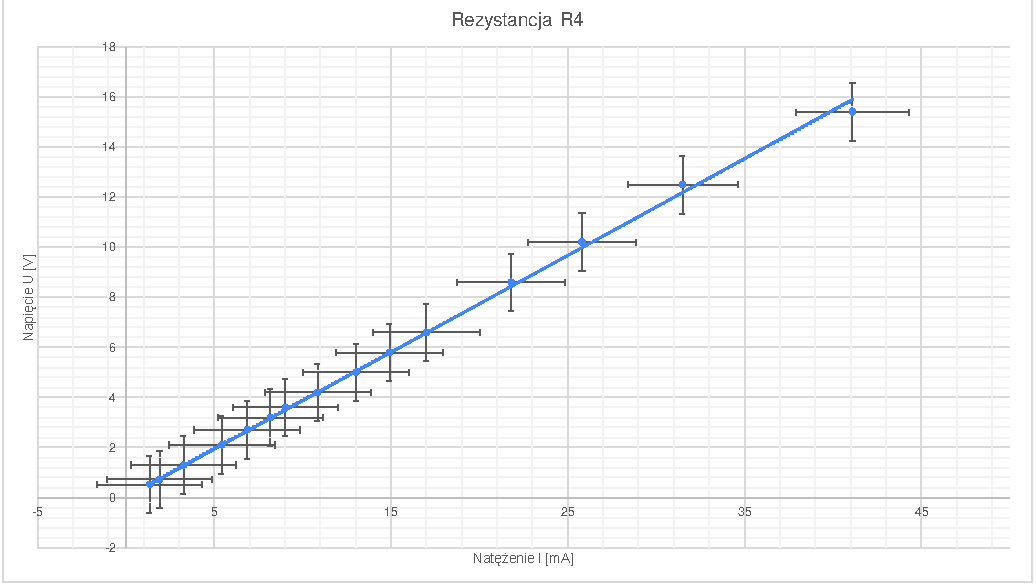
\includegraphics[scale=0.65]{Wykres1.pdf}
\caption{Wykres pomiarów napięcia i natężenia wraz z linią dopasowania}
\end{figure}

\end{document}
